\documentclass[11pt]{article}

% Package Header

\usepackage[paperheight=11in,
			paperwidth=8.5in,
			inner=0.4in,
			textheight=8.9in,
			textwidth=7.8in,
			marginparwidth=120pt,
			marginparsep=32pt,
			bottom=1.4in,
			footskip=1.0in]{geometry}
\geometry{letterpaper}                   % ... or a4paper or a5paper or ...

\usepackage{array}
\usepackage{amssymb}
\usepackage{asymptote}
\usepackage{amsmath}
\usepackage{amsfonts}
\usepackage{animate}
\usepackage{arrayjobx}
\usepackage{arydshln}
\usepackage{bookman}
\usepackage{color}
%\usepackage{colortbl}
\usepackage{cancel}
\usepackage{calculator}
\usepackage{collcell}
\usepackage{epstopdf}
\usepackage{enumerate}
\usepackage{epsfig}
%\usepackage{etex}
\usepackage[english]{babel}
\usepackage{etoolbox}
% \usepackage{fancyhdr}
\usepackage{fancybox}
\usepackage[nomessages]{fp}
\usepackage{graphics}
\usepackage{graphicx}
\usepackage{ifthen}
\usepackage{ifmtarg}
\usepackage[latin1]{inputenc}
\usepackage{latexsym}
\usepackage{multirow}
\usepackage{multicol}
\usepackage{multimedia}
\RequirePackage[noplaybutton]{media9}
\usepackage{mathbbol}
\usepackage{mathtools}
\usepackage{multido}
\usepackage{palatino}
\usepackage{polynom}
\usepackage{pxfonts}
\usepackage{pifont}
\usepackage{pgffor}
%\usepackage{pgfplots}
\usepackage{pdfpages}
\usepackage[parfill]{parskip}
\usepackage{soul}
\usepackage{tikz}
\usetikzlibrary{arrows,shapes,trees,shapes.geometric,calc}
\usepackage{txfonts}
\usepackage{tcolorbox}
\usepackage{wasysym}
\usepackage{wrapfig}
\usepackage{xcolor}
\usepackage{xmpmulti}
\usepackage{xparse}
\usepackage{xstring}
\usepackage{enumitem}

%\usepackage{hyperref}
\usepackage{geometry}
\usepackage{amsmath}
\usepackage{amssymb}
\usepackage{amsthm}
\usepackage{amscd}
\usepackage{amsfonts}
\usepackage{graphicx}%
\usepackage{fancyhdr}
\usepackage{array}
\usepackage{pgf,tikz}
\usetikzlibrary{arrows}

% Uncomment the following lines to use the Palatino font.  Remove the
% [osf] bit if you don't like the old style figures.

%\usepackage[T1]{fontenc}
\usepackage[osf]{mathpazo}
%\usepackage{mathpazo}

% Set your name here
%\def\name{Geoffrey W. Cox}

% The following metadata will show up in the PDF properties
%\hypersetup{
%  colorlinks = true,
%  urlcolor = black,
%  pdfauthor = {\name},
%  pdfkeywords = {economics empirical industrial organization econometrics
%    microeconomics applied microeconomics},
%  pdftitle = {\name: Curriculum Vitae},
%  pdfsubject = {Curriculum Vitae},
%  pdfpagemode = UseNone
%}

\geometry{textheight=9.0in, textwidth=6in}

%% Customize page headers
%\pagestyle{myheadings}
%\markright{\name}
%\thispagestyle{empty}

% Customize section headings
\usepackage{sectsty}
\subsectionfont{\rmfamily\mdseries\itshape\large}

% Don't indent paragraphs.
\setlength\parindent{0em}

% Make lists without bullets
\renewenvironment{itemize}{
  \begin{list}{}{
    \setlength{\leftmargin}{1em}
  }
}{
  \end{list}
}

\pagestyle{fancy}\lhead{Written Homework 07} \rhead{Due Mar 12}
\chead{{\large{\bf Divergence Theorem}}} \lfoot{} \rfoot{\bf \thepage} \cfoot{}

\begin{document}

\newcommand{\NP}{\newpage\thispagestyle{empty}}
\newcommand{\B}{\textcolor{blue}}
\newcommand{\R}{\textcolor{red}}
\newcommand{\G}{\textcolor{olive}}
\newcommand{\Or}{\textcolor{YellowOrange}}
\newcommand{\DEF}{\underline{Defn}:\ \ \ }
\newcommand{\THM}{\underline{Thm}:\ \ \ }
\newcommand{\PROP}{\underline{Properties}:\ \ \ }
\newcommand{\NOTE}{\underline{Notes}:\ \ \ }
\newcommand{\EX}{\underline{Ex}:\ \ \ }
\newcommand{\SOL}{\underline{Soln}:\ \ \ }
\newcommand{\UL}{\underline}
\newcommand{\RE}{\mathbf{R}}
\newcommand{\V}{\textbf{ v }}
\newcommand{\VV}{[v_1,v_2]}
\newcommand{\VVV}{[v_1,v_2,v_3]}
\newcommand{\W}{\textbf{ w }}
\newcommand{\WW}{[w_1,w_2]}
\newcommand{\WWW}{[w_1,w_2,w_3]}
\newcommand{\VA}{\textbf{ a }}
%\newcommand{\AA}{[a_1,a_2]}
\newcommand{\AAA}{[a_1,a_2,a_3]}
\newcommand{\VB}{\textbf{ b }}
\newcommand{\BB}{[b_1,b_2]}
\newcommand{\BBB}{[b_1,b_2,b_3]}
\newcommand{\VC}{\textbf{ c }}
\newcommand{\CC}{[c_1,c_2]}
\newcommand{\CCC}{[c_1,c_2,c_3]}
\newcommand{\VI}{\textbf{ i }}
\newcommand{\VJ}{\textbf{ j }}
\newcommand{\VK}{\textbf{ k }}
\newcommand{\VF}{\textbf{ F }}
\newcommand{\VG}{\textbf{ G }}
\newcommand{\VO}{{\vec{0}}}
\newcommand{\OBUL}{\quad $\circ$ \ \ \ }
\newcommand{\NEWLINE}{\\ \hspace{0.63cm}}
\newcommand{\CAN}{\cancel}
\newcommand{\GF}{{\nabla f}}
\newcommand{\PFPX}{{\dfrac{\partial f}{\partial x}}}
\newcommand{\PFPY}{{\dfrac{\partial f}{\partial y}}}
\newcommand{\PFPZ}{{\dfrac{\partial f}{\partial z}}}
\newcommand{\DFDX}{{\dfrac{df}{dx}}}
\newcommand{\GG}{{\nabla g}}
\newcommand{\PGPX}{{\dfrac{\partial g}{\partial x}}}
\newcommand{\PGPY}{{\dfrac{\partial g}{\partial y}}}
\newcommand{\PGPZ}{{\dfrac{\partial g}{\partial z}}}
\newcommand{\DGDX}{{\dfrac{dg}{dx}}}
\newcommand{\PPX}{{\dfrac{\partial}{\partial x}}}
\newcommand{\PPY}{{\dfrac{\partial}{\partial y}}}
\newcommand{\PPZ}{{\dfrac{\partial}{\partial z}}}
\newcommand{\PP}{\partial}
\newcommand{\DELF}{\nabla \cdot \textbf{ F }}
\newcommand{\CURLF}{\nabla \times \textbf{ F }}
\newcommand{\DEL}{\nabla \cdot }
\newcommand{\CURL}{\nabla \times }
\newcommand{\RT}{\textbf{ r }(t)}
\newcommand{\RPT}{\textbf{ r }'(t)}
\newcommand{\GINT}{\iint \limits_{R} (\text{curl} \ \textbf{ F }) \cdot \textbf{ k } \ dA}
\newcommand{\ON}{\onslide}
\newcommand{\OB}{\overbrace}
\newcommand{\OBT}{\overbracket}
\newcommand{\OS}{\overset}
\newcommand{\UB}{\underbrace}
\newcommand{\UBT}{\underbracket}
\newcommand{\US}{\underset}
\newcommand{\D}{\displaystyle}
\newcommand{\MCol}{\multicolumn}
\newcommand{\RRE}{\mathbf{R}^2}
\newcommand{\RRRE}{\mathbf{R}^3}
\newcommand{\DXDT}{{\dfrac{dx}{dt}}}
\newcommand{\DYDT}{{\dfrac{dy}{dt}}}
\newcommand{\DZDT}{{\dfrac{dz}{dt}}}
\newcommand{\FRT}{\textbf{ F }(\textbf{ r }(t))}
\newcommand{\WORK}{ {\int \limits_{C} \textbf{ F } \cdot d\textbf{ r }} }
\newcommand{\WORKAB}{ {\int \limits_{A}^{B}\textbf{ F } \cdot d\textbf{ r }} }
\newcommand{\WORKT}{ {\int \limits_{a}^{b}\textbf{ F }(\textbf{ r }(t)) \cdot \textbf{ r }'(t) \ dt} }
\newcommand{\FLUX}{ {\iint \limits_{S}\textbf{ F } \cdot d\textbf{ S }} }
\newcommand{\FLUXX}{ {\iint \limits_{S}\textbf{ F } \cdot \textbf{ n } \ dS} }
\newcommand{\FLUXXX}{ {\iint \limits_{R}\textbf{ F }(\textbf{ r }(u,v)) \cdot \textbf{ N } \ du\ dv} }
\newcommand{\OWORK}{ {\oint \limits_{C}\textbf{ F } \cdot d\textbf{ r }} }
\newcommand{\GREENT}{ {\oint \limits_{C}\textbf{ F }\cdot \textbf{ T } \ ds} }
\newcommand{\GREENN}{ {\oint \limits_{C}\textbf{ F }\cdot \textbf{ N } \ ds} }
\newcommand{\DIVTHM}{\iiint \limits_{T} \text{div} \ \textbf{ F }  \ dV}
\newcommand{\GREENCURL}{\iint \limits_{R} (\text{curl} \ \textbf{ F }) \cdot \textbf{ k } \ dA}
\newcommand{\STOKECURL}{\iint \limits_{S} (\text{curl} \ \textbf{ F }) \cdot \textbf{ n } \ dS}
\newcommand{\GREENDIV}{\iint \limits_{R} \text{div} \ \textbf{ F } \ dA}
\newcommand{\GREENSA}{\iint \limits_{R} \left(\dfrac{\partial N}{\partial x} - \dfrac{\partial M}{\partial y}\right) \ dA}
\newcommand{\GREENSL}{\oint \limits_{C} (M\ dx + N\ dy )}
\newcommand{\FDR}{ {\textbf{ F } \cdot d\textbf{ r }} }
\newcommand{\FDRT}{ {\textbf{ F }(\textbf{ r }(t)) \cdot \textbf{ r }'(t)} }
\newcommand{\BCOLS}{\begin{columns}}
\newcommand{\BCOL}{\begin{column}}
\newcommand{\ECOLS}{\end{columns}}
\newcommand{\ECOL}{\end{column}}
\newcommand{\BLINE}{\tikz[baseline]}
\newcommand{\NODERRB}{\node[fill=red!10,draw,rectangle,anchor=base]}
\newcommand{\NODEGRB}{\node[fill=green!10,draw,rectangle,anchor=base]}
\newcommand{\NODEBRB}{\node[fill=blue!10,draw,rectangle,anchor=base]}
\newcommand{\NODECRB}{\node[fill=red!0,draw,rectangle,anchor=base]}
\newcommand{\NODERR}{\node[fill=red!10,rectangle,anchor=base]}
\newcommand{\NODEGR}{\node[fill=green!10,rectangle,anchor=base]}
\newcommand{\NODEBR}{\node[fill=blue!10,rectangle,anchor=base]}
\newcommand{\NODECR}{\node[fill=red!0,rectangle,anchor=base]}
\newcommand{\NODERE}{\node[fill=red!10,draw,ellipse,anchor=base]}
\newcommand{\NODEGE}{\node[fill=green!10,draw,ellipse,anchor=base]}
\newcommand{\NODEBE}{\node[fill=blue!10,draw,ellipse,anchor=base]}
\newcommand{\NODECE}{\node[fill=red!0,draw,ellipse,anchor=base]}
\newcommand{\NODERC}{\node[fill=red!10,draw,circle,anchor=base]}
\newcommand{\NODEGC}{\node[fill=green!10,draw,circle,anchor=base]}
\newcommand{\NODEBC}{\node[fill=blue!10,draw,circle,anchor=base]}
\newcommand{\NODECC}{\node[fill=blue!0,draw,circle,anchor=base]}
\newcommand{\CNODE}{\tikz[na]\node [coordinate] }
\newcommand{\BENDL}{edge [bend left] }
\newcommand{\BENDR}{edge [bend right] }
\newcommand{\ARROWR}{\path [red,->]}
\newcommand{\ARROWG}{\path [green,->]}
\newcommand{\ARROWB}{\path [blue,->]}
\newcommand{\ARROWSR}{\path [red,<->]}
\newcommand{\ARROWSG}{\path [green,<->]}
\newcommand{\ARROWSB}{\path [blue,<->]}
\newcommand{\LINER}{\path [red,-]}
\newcommand{\LINEG}{\path [green,--]}
\newcommand{\LINEB}{\path [blue,--]}
\newcommand{\DE}{east}
\newcommand{\DW}{west}
\newcommand{\DN}{north}
\newcommand{\DS}{south}

\newcommand{\TT}[1]{\texttt{#1}}

\tikzstyle{every picture}+=[remember picture]
\tikzstyle{na} = [baseline=-1.5ex]

%%-----------------------------------------------------------
%% Bliss Definitions
\newcommand{\To}{\Rightarrow}
\newcommand{\del}{\nabla}
\newcommand{\C}{\mathcal{C}}
\newcommand{\N}{\mathcal{N}}
\newcommand{\A}{\mathcal{A}}
\renewcommand{\O}{\mathcal{O}}
% \renewcommand{\N}{\mathbb{N}}
\newcommand{\ben}{\begin{enumerate}}
\newcommand{\een}{\end{enumerate}}
\newcommand{\eps}{\varepsilon}
\renewcommand{\epsilon}{\varepsilon}
\newcommand{\p}{\partial}
\newcommand{\<}{\langle}
\renewcommand{\>}{\rangle}
\renewcommand{\subset}{\subseteq}
\newcommand{\cont}{\Rightarrow \Leftarrow}
\newcommand{\back}{\backslash}
\newcommand{\abs}[1]{|{#1}|}
\newcommand{\ip}[1]{\langle{#1}\rangle}
\newcommand{\m}[1]{{\mathbf{#1}}}
\newcommand{\sts}{\m{S}^\textrm{T}\m{S}}
\newcommand{\rank}{\textrm{rank}}
\newcommand{\X}{\mathcal{X}}
\newcommand{\Y}{\mathcal{Y}}
\def\ds{\displaystyle}
\def\d{\partial}
\renewcommand{\arraystretch}{1.5}
%%-----------------------------------------------------------


\newcommand\CEN[1]{\multicolumn{1}{c}{ #1 }}

\newcommand\MATL[3]
{{%
\arraycolsep=#1\arraycolsep\ensuremath{{\setlength{\extrarowheight}{#2cm}\begin{bmatrix*}[l]#3\end{bmatrix*}}}
}}
\newcommand\MATC[3]
{{%
\arraycolsep=#1\arraycolsep\ensuremath{{\setlength{\extrarowheight}{#2cm}\begin{bmatrix*}[c]#3\end{bmatrix*}}}
}}
\newcommand\MATR[3]
{{%
\arraycolsep=#1\arraycolsep\ensuremath{{\setlength{\extrarowheight}{#2cm}\begin{bmatrix*}[r]#3\end{bmatrix*}}}
}}

\newcommand\MATDL[3]
{{%
\arraycolsep=#1\arraycolsep\ensuremath{{\setlength{\extrarowheight}{#2cm}\begin{vmatrix*}[l]#3\end{vmatrix*}}}
}}
\newcommand\MATDC[3]
{{%
\arraycolsep=#1\arraycolsep\ensuremath{{\setlength{\extrarowheight}{#2cm}\begin{vmatrix*}[c]#3\end{vmatrix*}}}
}}
\newcommand\MATDR[3]
{{%
\arraycolsep=#1\arraycolsep\ensuremath{{\setlength{\extrarowheight}{#2cm}\begin{vmatrix*}[r]#3\end{vmatrix*}}}
}}

\newcommand\TABwB[3]
{{
\setlength{\extrarowheight}{#1 cm}
\begin{tabular}{#2}
	\hline
	#3
	\hline
\end{tabular}
}}

\newcommand\TABwoB[3]
{{
\setlength{\extrarowheight}{#1cm}
\begin{tabular}{#2}
	#3
\end{tabular}
}}

\newcommand\includegraphicsDD[2]
{%
\includegraphics[scale=#1]{#2}
}

\newcommand\includegraphicsDDD[2]
{%
\includemedia[scale=#1,3Dmenu,activate=onclick,deactivate=onclick,
3Droll=0.,
3Dortho=0.0046491301618516445,
3Dc2c=0.8617081642150879 -0.29301872849464417 0.4142450988292694,
3Dcoo=-13.165555000305176 3.489872455596924 52.97535705566406,
3Droo=149.99999574342704,
3Dlights=Headlamp,add3Djscript=asylabels.js]{\includegraphics{#2}}
{#2.prc}
}

\newcommand\MATS[2]
{{%
  \arraycolsep=#1\arraycolsep\ensuremath{\begin{bmatrix*}[r]#2\end{bmatrix*}}
}}

\newcommand{\OKFACE}{
\begin{tikzpicture}
\draw[thick] (0cm,0cm) circle(.2cm);
\draw[thick] (-0.1,-0.09) -- (0.1,-0.09);
\draw [thick, fill=black] (0,0) circle (0.01);
\draw [rotate=90, fill=white] (0.06,0.06) circle (0.03);
\draw [rotate=90, fill=white] (0.06,-0.06) circle (0.03);
\end{tikzpicture}
}

\newcommand{\HAPPYFACE}{
\begin{tikzpicture}
\draw[thick] (0cm,0cm) circle(.2cm);
\draw[thick] plot [smooth,tension=1.5] coordinates{(-0.1,-0.08) (0,-0.13) (0.1,-0.08)};
\draw [thick, fill=black] (0,0) circle (0.01);
\draw [rotate=90, fill=white] (0.06,0.06) circle (0.04);
\draw [rotate=90, fill=white] (0.06,-0.06) circle (0.04);
\end{tikzpicture}
}

\newcommand{\SADFACE}{
\begin{tikzpicture}
\draw[thick] (0cm,0cm) circle(.2cm);
\draw[thick] plot [smooth,tension=1.5] coordinates{(-0.1,-0.12) (0,-0.07) (0.1,-0.12)};
\draw [thick, fill=black] (0,0) circle (0.01);
\draw [rotate=90, fill=white] (0.06,0.06) circle (0.02);
\draw [rotate=90, fill=white] (0.06,-0.06) circle (0.02);
\end{tikzpicture}
}

\newcommand{\CounterReset}{
\setcounter{CritCounter}{1}
\setcounter{TestCounter}{1}
\setcounter{ColorCounter}{1}
\setcounter{Index}{1}
}

\newcommand\CritLineInitialize[1]{
\ifdef{\SymFun}
{
	\setcounter{CritLineSlide}{#1}
}
{
	\newarray\TestPts
	\newarray\TestVals
	\newarray\TestEVal
	\newarray\fIncDec
	\newarray\testsigns
	\newarray\inequality
	\setcounter{CritLineSlide}{#1}
	\newcommand\SymFun{}
	\newcommand\IncDecStr{}
	\newcommand\TestSignStr{}
	\newcommand\InEqStr{}
	\newcommand\SymFunD{}
	\newcommand\SymFunDLt{}
	\newcommand\SymFunN{}
	\newcommand\SymFunNLt{}
	\newcommand{\CritLineTable}{}
}
}

\newcommand\USubInitialize{
	\newcommand{\Fun}{}
	\newcommand{\FunN}{}
	\newcommand{\FunD}{}
	\newcommand{\FunU}{}
	\newcommand{\UIntegrand}{}
	\newcommand{\AFunU}{}
	\newcommand{\DX}{}
}

\newcommand*\circled[1]{\tikz[baseline=(char.base)]{
            \node[shape=circle,draw,inner sep=1pt,color=blue] (char) {#1};}}

\newcommand*\ellipsed[1]{\tikz[baseline=(char.base)]{
            \node[shape=ellipse,draw,inner sep=1pt,color=blue] (char) {#1};}}

\newcommand*\rected[1]{\tikz[baseline=(char.base)]{
            \node[shape=rectangle,draw,inner sep=1pt,color=blue] (char) {#1};}}

\newcommand*\starred[1]{\tikz[baseline=(char.base)]{
            \node[shape=star,star points=10,draw,inner sep=1pt,color=blue] (char) {#1};}}

\newcommand\CHECKBOX[1]{\makebox[0pt][l]{$\square$}\raisebox{.15ex}{\hspace{0.1em}\ON#1{\B{$\checkmark$}}}}

\makeatletter
\newcommand{\@RemovePositiveSignIfAny}[1]{\IfBeginWith{#1}{+}{\StrGobbleLeft{#1}{1}}{#1}}%
\newcommand{\@PlusIfNonZero}[1]{\IfStrEq{#1}{}{}{+}}%
\newlength{\@MySystemWidth}%
\newcommand*{\@ChooseSignWithAlignment}[2]{%
    \IfBeginWith{#2}{-}%
    {{}-\makebox[\@MySystemWidth][#1]{\ensuremath{\StrGobbleLeft{#2}{1}}}}%
    {{}\@PlusIfNonZero{#2}\makebox[\@MySystemWidth][#1]{\ensuremath{\@RemovePositiveSignIfAny{#2}}}}%
}%
\newcommand*{\@ChooseSignWithRightAlignment}[1]{\@ChooseSignWithAlignment{r}{#1}}%
\newcommand*{\@ChooseSignWithLeftAlignment}[1]{\@ChooseSignWithAlignment{l}{#1}}%

\newenvironment{MySystem}[3][1.2em]{% [<width>] {num of variables} {alignment}
    \newcolumntype{R}{>{\collectcell\@ChooseSignWithRightAlignment}{r}<{\endcollectcell}}
    \newcolumntype{L}{>{\collectcell\@ChooseSignWithLeftAlignment}{l}<{\endcollectcell}}
    \setlength{\@MySystemWidth}{#1}% Store the width to use to typeset the terms
    \IfStrEqCase{#3}{%
        {R}{\begin{array}{r@{} *{\numexpr#2-1\relax}{#3@{}} @{{}={}} r}}%
        {L}{\begin{array}{l@{} *{\numexpr#2-1\relax}{#3@{}} @{{}={}} l}}%
    }[\parbox{\linewidth}{\color{red}MySystem Error: Only L and R alignment types are supported. (using R)}\begin{array}{r *{\numexpr#2-1\relax}{#3} @{{}={}} r}]%
}{%
    \end{array}%
}
\newenvironment{MySystemNoEqual}[3][1.2em]{% [<width>] {num of variables} {alignment}
    \newcolumntype{R}{>{\collectcell\@ChooseSignWithRightAlignment}{r}<{\endcollectcell}}
    \newcolumntype{L}{>{\collectcell\@ChooseSignWithLeftAlignment}{l}<{\endcollectcell}}
    \setlength{\@MySystemWidth}{#1}% Store the width to use to typeset the terms
    \IfStrEqCase{#3}{%
        {R}{\begin{array}{r@{} *{\numexpr#2\relax}{#3@{}} @{{}{}} r}}%
        {L}{\begin{array}{l@{} *{\numexpr#2\relax}{#3@{}} @{{}{}} l}}%
    }[\parbox{\linewidth}{\color{red}MySystem Error: Only L and R alignment types are supported. (using R)}\begin{array}{r *{\numexpr#2\relax}{#3} @{{}{}} r}]%
}{%
    \end{array}%
}

\makeatother


In addition to the online homework, please hand in the following problems:

\vspace{0.2cm}

{\bf Problem 1:} Compute the outward flux of the following vector fields through the given solids:

%-------NUM LIST---------
\begin{enumerate}
	\item[a.] $\D{{\bf F} = [x^2,y^2,z^2]}$ where T is the solid cube in the first octant between the planes $\D{x = 1, \,y = 1,}$ and \, $\D{z = 1}$.
	
	\vspace{0.2cm}
	
	\item[b.] $\D{{\bf F} = x^3\,{\bf i} + y^3\,{\bf j} + z^3\,{\bf k}}$ where T is the solid sphere: $\D{x^2 + y^2 + z^2 \le 9}$
	
	\vspace{0.2cm}
	
	\item[c.] $\D{{\bf F} = [6x^2+2xy,\,2y+x^2z,\,4x^2y^3]}$ where T is the solid cylinder $\D{x^2 + y^2 = 4}$ \,  between the planes $z=0$ and $z=3$.
	
\end{enumerate}
%------------------------I

\vspace{0.2cm}

{\bf Problem 2:} Let ${\bf F} = x{\bf i} + y{\bf j} + z{\bf k}$ and suppose that the surface S and region D satisfy the hypotheses of the Divergence Theorem. Show that the volume of D is given by the formula

\begin{center}
	Volume of D = $\D{\frac{1}{3} \iint \limits_{S} {\bf F} \cdot {\bf n}\, dA}$
\end{center}

\vspace{0.2cm}

{\bf Problem 3:} The the closed cube-like surface, $S$, shown below has a top that is an unknown smooth surface. Let ${\bf F} = (5x+2){\bf i} - 7y{\bf j} + 7z{\bf k}$. Suppose we knew the outward flux through sides $C$ and $B$ were both $-4$,the volume of the solid is 10 and the area of $A$ is 4.  Find the outward flux through the top?	

\begin{center}
	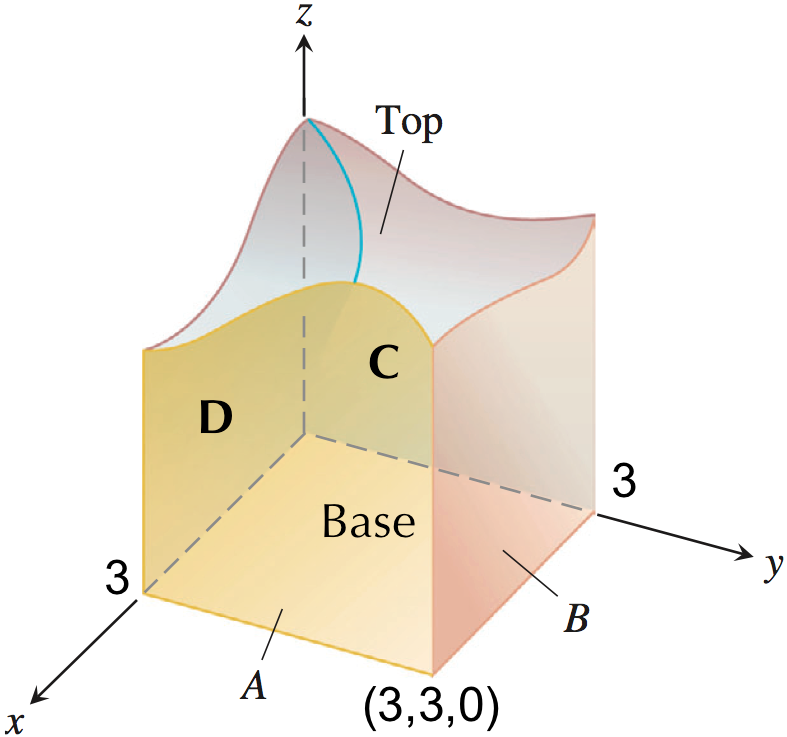
\includegraphics[scale = 0.2]{HWFigs/HW10_fig1.png}
\end{center}

\vspace{0.2cm}

{\bf Problem 4:} Show that the outward flux of a constant vector field {\bf F} across any closed surface is zero.


%\thispagestyle{empty}
%\newpage
%\thispagestyle{empty}


\end{document}